\chapter{并行化加速的预条件共轭梯度算法}
\label{cha:algo}

\section{供电网络的抽象数学模型}

由于本数据集是瞬态的直流DC网络,所以网络中只有三种基本元件:电阻、独立电压源、独立电流源。为了建立改进节点分析方法的方程,先根据
电路里的连接关系建立系数矩阵$A$:对于连接节点$i$与节点$j$的支路$k$,如果这个支路的方向是从$i$到$j$,那么$A_{k,i}=1, A_{k,j}=-1$;
如果支路的方向是从$j$到$i$,那么$A_{k,i}=-1, A_{k,j}=1$;其余情况$A$的元素为0。

更进一步的,根据支路$b$是纯电阻支路、电压源支路、电流源支路可以把$A$按列分成三部分$A_G,A_V,A_I$。同样的对于支路电流向量$i$,可以分成$i_G,i_V,i_I$;
对于节点电压向量$v_b$,可以分成$v_G,v_V,v_I$。
\begin{align}
A=\begin{bmatrix} A_I \\ A_V \\ A_G \end{bmatrix}, \quad
i_b=\begin{bmatrix} i_I \\ i_V \\ i_G \end{bmatrix},\quad
v_b=\begin{bmatrix} v_I \\ v_V \\ v_G \end{bmatrix}
\end{align}
那么根据基尔霍夫电压定律和基尔霍夫电流定律可以写出($v_n$是节点电压向量):
\begin{align}
A^T i_b & =  0 \\
A v_n & = v_b
\end{align}
展开上述两个式子可得:
\begin{align*}
A_I^T i_I + A_V^T i_V + A_G^T i_G & = 0 \\
A_I v_n & = v_I \\
A_V v_n & = v_V \\
A_G v_G & = v_G \\
i_I & = I \\
v_V & = V \\
i_G & = P v_G \\
\end{align*}
其中$P$是电导邻接矩阵:如果支路$k$上存在阻值为$R$、连接$i$到$j$的电阻,那么$P_{k,i}=\frac{1}{R}$,$P_{k,j}=\frac{1}{R}$。

根据改进节点分析方法的原理,可以通过简化去掉所有支路电压的变量,也就是$v_b$;以及大部分支路电流变量,也就是$i_b$。
化简后可以得到:
\begin{align}
    A_G^T P A_G v_n + A_V^T i_V & = -A_I^T I    \\
    A_V v_n & =V
\end{align}
令$G=A_G^T P A_G$,其中$G$也就是在公式\ref{Geq}中提到的电导矩阵。那么可以得到:
\begin{align}
    \begin{bmatrix}
    G & A_V^T \\
    A_V & 0 \\
    \end{bmatrix}
    \begin{bmatrix}
    v_n \\ i_V
    \end{bmatrix}
    =
    \begin{bmatrix}
    0 & -A_I^T  \\
    1 & 0
    \end{bmatrix}
    \begin{bmatrix}
    V \\ I
    \end{bmatrix}
    \label{eqbasic}
\end{align}

式\ref{eqbasic}的右边是确定的,左边有一个未知向量$x=\begin{bmatrix}v_n \\ i_V\end{bmatrix}$,因此可以使用线性方程求解器进行求解。此外,系数矩阵
可以看出来非常稀疏并且是对角占优的,因此有很多优化的余地。但是,值得注意的是系数矩阵并不是对称正定的,所以像Cholesky Solver这种算法就不能再用了。

\subsection{处理节点间的短路}

由于系数矩阵使用的是电导值,所以节点间的短路并不能直接用阻值为0的电阻代替。为了解决这个问题,考虑对于一个电路来说,由短路的节点组成的集合等效于一个超节点,也就是说
我们可以把它们当做一个节点来处理。实现的时候,对于短路的节点集合,我们新建一个超节点表示它们的等效节点,与这个超节点相连的所有支路是这些短路的节点的支路的并集,这个
超节点挂载的电流源负载是这些短路的节点的电流源负载之和。

此外,为了求出超节点,在处理读入数据的时候,我们采用了并查集~\cite{tarjan1975efficiency}的方法,即维护一个图的森林,一开始所有节点都是森林里的孤立的节点;如果读入两个节点$i$和$j$是短路的,那么找到节点$i$所在的连通块的根节点,把这个根节点挂在节点$j$下,也就是成为$j$的子节点;最后所有节点的关系形成了一个森林,森林里每个连通块都是
一个超节点。

\section{解线性方程的共轭梯度算法}

求解式\ref{eqbasic}中的线性方程组有两种基本方法:直接求解法与间接迭代法。直接求解法的算法鲁棒性更强,但是由于该线性方程组的节点规模非常巨大,直接求解法会要求
过多的CPU计算资源与内存,无法解决问题。迭代法由于预条件子的问题,求解稳定性不如直接求解法,但是更加节省计算资源,是解决该问题的合适方法。对于本问题,我们采取经典的基于预条件子的共轭梯度法(Preconditioned Conjugate Gradient Method,PCG)进行求解。下文探讨的主要是对此算法的优化。

没有用预条件子的共轭梯度算法如下所示:
\begin{lstlisting}
//算法1.cpp
r[0] = b - A * x0;
p[0] = r[0];
k = 0;
repeat
    alpha[k] = dot(r[k], r[k]) / dot(p[k], A * p[k]);
    x[k+1] = x[k] + alpha[k] * p[k];
    r[k+1] = r[k] - alpha[k] * A * p[k];
    if r[k+1]足够小
        break;
    else
        beta[k] = dot(r[k+1], r[k+1]) / dot(r[k], r[k]);
        p[k+1] = r[k+1] + beta[k] * p[k];
        k = k + 1;
    end if
end until
求解结果为x[k+1]
\end{lstlisting}

但是共轭梯度算法的求解速度,也就是收敛速度取决于系数矩阵$A$的条件数。为了改善这一点,我们可以用一个预条件子$M$对系数矩阵$A$进行预处理,使得$M^{-1}A$的条件数尽量小。
使用预条件子后的算法如下:
\begin{lstlisting}
//算法2.cpp
r[0] = b - A * x0;
z[0] = inverse(M) * r[0]
p[0] = z[0];
k = 0;
repeat
    alpha[k] = dot(r[k], z[k]) / dot(p[k], A * p[k]);
    x[k+1] = x[k] + alpha[k] * p[k];
    r[k+1] = r[k] - alpha[k] * A * p[k];
    if r[k+1]足够小
        break;
    else
        z[k+1] = inverse(M) * r[k+1];
        beta[k] = dot(z[k+1], z[k+1]) / dot(z[k], z[k]);
        p[k+1] = z[k+1] + beta[k] * p[k];
        k = k + 1;
    end if
end until
求解结果为x[k+1]
\end{lstlisting}

\section{基于多重网格的预条件子}

多重网格方法~\cite{trottenberg2000multigrid}(Multigrid Method)是非常有效的预条件子算法。它的核心思想是,在不同粗粒度的维度进行迭代计算,从而对各种频率的误差进行消除。
本文的算法使用多重网格来改善共轭梯度算法的收敛速度;因为迭代算法的迭代过程是强数据依赖的,无法进行并行加速,所以收敛性的提高有助于算法效率的提升。

为了介绍多重网格方法,先引入以下概念:给定一个线性方程组$Ax=b$和一个初始解$x_0$,一个迭代解法具有以下的形式:
\begin{align}
    x_{k+1} = x_k + M^{-1} (b-Ax_k)
    \label{eq:iter}
\end{align}
其中$k$是迭代轮数的编号,$x_k$是第$k$轮迭代的近似解,$M$是预条件子,$M^{-1}A$的条件数应该尽量小。设$\hat{x}$为方程组的精确解,则$e=x-\hat{x}$是迭代解与
精确解之差,可以证明~\cite{briggs2000multigrid}$e$可以表达为低频与高频的傅里叶分量之和。更重要的是,Briggs等人~\cite{briggs2000multigrid}指出,传统的迭代方法
(如高斯-赛达尔迭代法,共轭梯度算法等)虽然能高效地移除$e$中的高频部分,但对低频部分的消除却十分缓慢。

为了弥补这一点的不足,多重网格方法引入了这两种操作:(1) 松弛平滑操作(Smoothing),用于降低误差中的高频部分;(2) 粗网格修正(Coarse Grid),用以降低误差中的低频部分。
松弛操作中,会运行若干轮的原始迭代算法,得到一个粗略的解$x_h$。粗网格修正中,会把原问题映射到一个规模更小的子问题上,在这个子问题中运用同样的方法进行求解,最后把解
回代到原问题中。在映射与逆映射中,最重要的是网格转换运算,即网格限制运算(Restriction Operator)与网格内插运算(Prolongation Operator)。

多重网格的一种常用实现是,从细网格(Fine Grid)开始,对其进行松弛平滑操作(式\ref{eq:iter})以消除误差的高频分量;然后把细网格映射到粗网格上,同样地进行松弛平滑操作,
这样细网格中的一部分低频分量被降低了;最后把粗网格上的解内插回细网格上,并做最后的松弛平滑操作。这种算法流程被称为V-循环算法。算法的伪代码如下:

\begin{enumerate}
\item 对$A_f x_f = b_f$进行$v_1$次迭代操作,得到细网格中的一个粗略解$x'_{f}$;
\item 对$R_f=(b_f - A_f * x'_{f})$进行网格限制操作即$R_c=\text{Restriction}(R_f)$,得到$R_c$;
\item 如果$R_c$所在的粗网格已经足够粗,也就是迭代深度超过预设值,那么跳转到第5步;
\item 否则令$x_c=0$,从第1步开始递归计算;
\item 设递归返回的结果是$x'_c$,那么用$x'_c$去修正$x'_f$的值,即$x'_f \leftarrow x'_f + \text{Prolongation}(x'_c)$;
\item 对修正过后的$x'_f$进行$v_2$次迭代操作,得到最终的迭代解。(如果是递归调用到达这一步的,那么返回到第5步)
\end{enumerate}
其中$v_1$与$v_2$的值根据经验一般设为2或3。

\section{多机并行优化中的线程级优化}

实现算法的时候,我们在两个方面进行了并行优化:线程级和进程级的优化。实验时使用具有八个核心(CPU Processor)的机器,我们在每个核心上使用八个线程并行进行各种矩阵运算,包括
向量内积、矩阵与向量的乘法、向量加法等,从而最大程度地发掘算法的并行性。

首先,为了进行线程级的优化,我们直接使用了OpenMP代码库提供的API。OpenMP(Open Multi-Processing)是支持多平台共享内存多线程编程的应用程序接口。接口中包括了一系列
编译指令、库函数以及环境变量,从而改变程序会影响运行时的表现。为了实现多线程并行,OpenMP会从主线程中派生出多个从线程,这些从线程一起执行可以安全并行的任务。
对于程序员来说,只需要在源代码中加入特定的编译指令,编译器就可以根据实际情况生成并行化的代码。

一个典型的例子如下:
\begin{lstlisting}
//dot_product.cpp
int ComputeDotProduct(const int n, const Vector & x, const Vector & y, double & result) {
  result = 0.0;
  double * xv = x.values;
  double * yv = y.values;
  #pragma omp parallel for reduction (+:result)
  for (local_int_t i=0; i<n; i++)
    result += xv[i]*yv[i];
  return 0;
}
\end{lstlisting}

上述例子中,通过pragma指令,我们实现了向量内积算法中的线程级并行化。实现的方法是在可以并行执行的循环代码前加pragma指令,这样编译器就会自动生成相应的代码,在循环代码前
派生出若干个线程,不同线程之间并行执行,执行完后汇集到父线程上。
需要注意的是,由于不同线程的计算累加结果是分开存储的,所以要在pragma指令中指明对result变量进行reduction操作,从而把所有线程计算的结果累加存储在result变量中。
使用OpenMP之前,要注意判断代码中是否有数据依赖的部分;如果有,要尽量去掉,保证代码的可并行性。

\section{多机并行优化中的进程级优化}

虽然上一小节中提到的线程级的优化对程序效率已经有了不少提升,但是还远远不够。因为线程级的并行化要求共享内存,也就是所有数据都存储在本机上;此外,单机的
处理能力是有限的,本实验的数据规模较大,需要更多的计算资源。为此,需要进行多机的并行化处理,也就是进程级的并行优化。进程级的并行加速能最大程度地同时发掘多台机器的
计算能力,非常适合解决这种大规模的计算问题。但是与线程级的优化不同,进程与进程之间的内存是不共享的,因此进程与进程之间需要相互通信,从而同步计算的数据。对于进程级
的并行化来说,通信带来的时间与空间开销往往限制了算法的优劣程度以及算法的并行化程度。通常来说,进程、机器越多,通讯的花销越大,性能有可能不如使用进程更少的算法。
\begin{figure}[H]
  \centering
  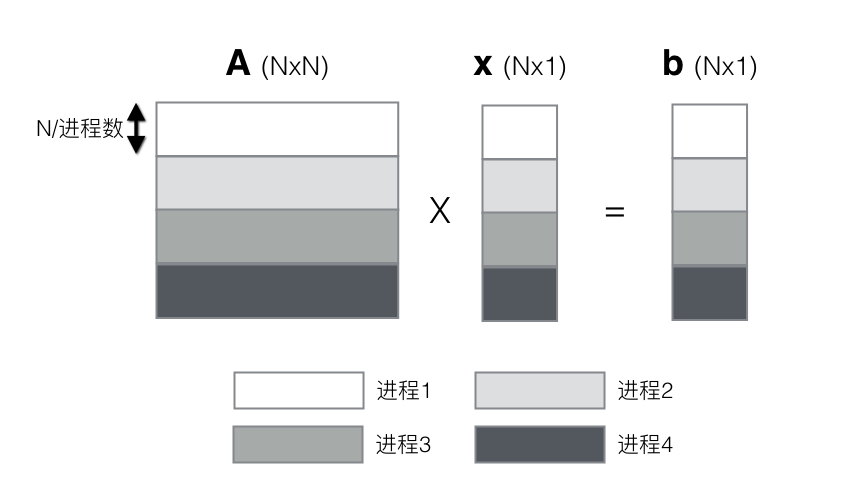
\includegraphics[height=8cm]{paral_demon}
  \caption{MPI中的负载平衡}
  \label{fig:figparaldemon}
\end{figure}

对于本实验来说,我们需要把进程的并行化运用到共轭梯度算法中。注意到系数矩阵非常稀疏,并且具有局部性。
那么一种可行的办法是把矩阵中连续的行分配给每一个进程,如图\ref{fig:figparaldemon}所示:若系数矩阵的
大小为$N\times N$,共有$K$个进程,那么第一个进程计算$x_1,\ldots,x_{\frac{N}{k}}$,第二个进程计算计算$x_{\frac{N}{k}+1},\ldots,x_{2\frac{N}{k}}$,
依次类推。也就是对于进程$i$来说,他只负责计算和保存$x_{(i-1)\frac{N}{k}+1},\ldots,x_{i\frac{N}{k}}$的值。所以在第$i$个进程迭代更新$x$的值的时候,需要
通过通讯手段来获得其余$x$(不在这个进程上)的值。在程序中,由于这一点,我们不能再用变量x来访问整个向量,因为内存中只存有该向量的部分内容(下文中用
local\_x来表示本地进程中的x的值)。为了正确地执行原算法,我们必须在进程中进行必要的通讯以交换不同进程的内容。

对于共轭梯度算法来说,主要的数学运算与对应的通讯方法如下:

\begin{itemize}
\item 计算向量$x$和$y$的内积。由于本进程中只有local\_x与local\_y的内容,所以每个进程先计算各自local\_x与local\_y的内积,存为local\_result,即本地结果;然后
把各自的本地结果广播给其他进程,从而完成本地结果的累加,计算出全局的内积;
\item 计算向量$x$和$y$的和。直接计算即可,不需要通讯,因为向量加法对于各个元素来说是独立的;
\item 计算矩阵$A$和向量$x$的乘积$y$。因为计算结果$y$是局部的,也就是只需要计算$y_{(i-1)\frac{N}{k}+1},\ldots,y_{i\frac{N}{k}}$,所以只需存储系数矩阵A的第
$((i-1)\frac{N}{k}+1)$到$(i\frac{N}{k})$行;此外,如果存在非零系数$A_{i,j}$,那么计算结果时就需要$x_j$的值;所以我们需要预处理出每一个$y_i$所需要的非局部的
$x$值,并通过通讯手段从其他进程中获取其值。
\end{itemize}

改动后的算法3如下:
\begin{lstlisting}
//算法3.cpp
local_r[0] = local_b - local_A * local_x0;
syncGlobal(sync_r, local_r);
local_z[0] = inverse(M) * sync_r[0];
local_p[0] = local_z[0];
k = 0;
repeat
    //get global dot(r,z)
    local_rtz = dot(local_r[k], local_z[k]);
    getGlobal(global_rtz, local_rtz);
    //get global dot(p,Ap)
    syncGlobal(sync_p, local_p);
    local_Ap = local_A * sync_p;
    local_pAp = dot(local_p[k], local_Ap);
    getGlobal(global_pAp, local_pAp);
    //compute alpha
    alpha[k] = global_rtz / global_pAp;
    //compute x
    local_x[k+1] = local_x[k] + alpha[k] * local_p[k];
    local_r[k+1] = local_r[k] - alpha[k] * local_Ap[k];
    if r[k+1]足够小
        break;
    else
        syncGlobal(sync_r, local_r)
        local_z[k+1] = inverse(M) * sync_r[k+1];
        beta[k] = global_rtz / old_rtz;
        old_rtz = global_rtz;
        local_p[k+1] = local_z[k+1] + beta[k] * local_p[k];
        k = k + 1;
    end if
end until
求解结果为x[k+1]
\end{lstlisting}
其中,主要的通讯函数有:
\begin{enumerate}
    \item getGlobal(global\_data, local\_data)函数,作用是通过通讯手段从其他进程中获取、接受它们各自的local\_data值,并统计到global\_data变量中(合并结果的
    方法有累加、取最大值、取最小值等);
    \item syncGlobal(result, local\_data)函数,作用是通过通讯手段,从其他进程中获取、接受local\_data对应的变量的部分全局值,并存在result变量中;
\end{enumerate}

与单机上的原算法相比,使用了多进程并行化优化的算法3在矩阵运算方面处理的数据规模更小,比如所处理的向量长度从原来的$N$降到了$N/\text{处理器数量}$,因此减少了程序的
数学运算量;并且,利用矩阵与向量运算的各元素独立性,不同的进程之间可以并行执行各种运算,因此大大提高了程序运行的时间利用率;但是算法引入了另外一种开销:通讯开销。比如
在计算向量内积时,需要等待所有进程都计算完本地局部内积后再相加,才可以得出总体的内积;在计算矩阵与向量的乘积时,需要从其它进程中接收某些非本地向量元素,也需要把本地的
向量元素发送到其它有需要的进程里。可以看出,进程数越多,算法的并行度越高,计算本地结果的效率越高,但是花在通讯上的花销会更大;进程数越少,算法并行度越低,但是通讯代价
会降低。

在本实验中,多机的并行通讯采用了消息传递接口(Message Passing Interface,MPI)的标准。MPI接口能维持一个虚拟的网络拓扑结构,并为一系列进程(
具体来说一个进程可能是一个计算节点、服务器、或者个人电脑)之间的交互提供基本的通讯函数。MPI是不依赖于语言的,协议的接口都一样,只是接口下的实现根据语言与系统有所不同。
目前流行的MPI库有OpenMPI,MPICH等。本实验中使用的是Intel为计算集群提供的基于ICC的Intel MPI库。

\section{本章小结}

本章介绍了供电网络的抽象数学模型的建立,以及解决其相应的线性方程组的方法。基于现有的共轭梯度算法,作者实现了多机多核并行的算法,并进一步分析了这个算法的性能。最后,为了提高算法的性能,作者又引入了基于多重网格的预条件子,从而解决了问题病态下的收敛速度的问题。
